\documentclass[a4paper,11pt]{article}
\usepackage[left=2.5cm, right=2.5cm, top=1.5cm, bottom=1.5cm]{geometry}
\usepackage{graphicx}
\usepackage{amssymb}
\usepackage{amsmath}
\usepackage[procnames]{listings}
\usepackage{xcolor}
\usepackage{hyperref}
\usepackage{multicol}
\usepackage{wrapfig}

\hypersetup{ %color attributes of citation, link, etc.
    colorlinks=true,
    linkcolor=blue,
    filecolor=gray,
    urlcolor=blue,
    citecolor=blue,
}

\setlength{\parindent}{0pt}

\newcommand{\matlab}{\textsc{Matlab}} %very important and totally necessary addition
\newcommand{\parallelsum}{\mathbin{\!/\mkern-5mu/\!}}

%'codify' text for snippets
\usepackage{xcolor}
\definecolor{codegray}{gray}{1}
\newcommand{\code}[1]{\colorbox{codegray}{\texttt{#1}}}

\definecolor{keywords}{RGB}{255,0,90}
\definecolor{comments}{RGB}{0,0,113}
\definecolor{p_red}{RGB}{160,0,0}
\definecolor{p_green}{RGB}{0,150,0} 
\lstset{language=Python, 
        basicstyle=\ttfamily\small, 
        keywordstyle=\color{keywords},
        commentstyle=\color{comments},
        stringstyle=\color{p_red},
        showstringspaces=false,
        identifierstyle=\color{p_green},
		procnamekeys={def,class}}

\graphicspath{ {./images/} }
           
\begin{document}
% \begin{multicols}{2}[]

\section{Lubricant Properties}

\begin{wrapfigure}{r}{0.4\textwidth}
    \vspace{-60pt}
    \hspace{8pt}
    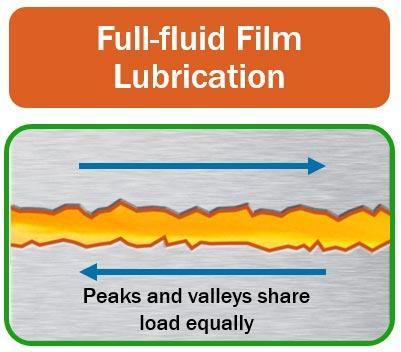
\includegraphics[width=0.9\linewidth]{film.jpeg} 
    \vspace{-10pt}
    \caption{Thin Film Lubrication}
    \vspace{-30pt}
    \label{film}
\end{wrapfigure}

Lubricants function by forming a thin barrier between two surfaces. When one surface moves across the other, this thin layer or film of lubricant will move freely with both surfaces to reduce the friction, this can be seen depicted in Figure \ref{film}. The following subsections will describe some of the key aspects of a well functioning lubricant.

\subsection{Viscosity}

The viscosity of the lubricant will determine the thickness of the film that is situated between the lubricated surfaces. Higher viscosity will ensure that the lubricated parts are separated and thereby reduce the mechanical wear on the components. This however will also increase the force required to move lubricated components and thereby lead to higher energy consumption losses and possibly heating of the components. A lower viscosity lubricant will incur lower energy losses and temperatures, however it might not form a film thick to sufficiently prevent mechanical wear, leading to the degradation of the surfaces. 

\subsection{Temperature \& Pressure Characteristics}

Lubricants are highly susceptible to temperature dependant and pressure dependant characteristic changes. These changes can greatly affect the functionality of the lubricant, and therefore must be taken into account when selecting a lubricant.


\subsubsection{Viscosity}

The viscosity of the particular lubricant will be highly dependant on the temperature and pressure it is operating at. As the temperature or the pressure of the operating lubricant increase the viscosity will decrease and vice versa. It is therefore important to select a lubricant that provides the correct viscosity at your applications temperature and pressure conditions. 

As the temperature of a lubricant decreases, there will come a point that is the coldest temperature that the lubricant will still flow. This temperature is known as the 'Pour Point' of the lubricant, for applications of lubricants at lower temperatures this value will dictate whether the lubricant will continue to function. 

\subsubsection{Volatility \& Flash/Fire point}

Lubricant volatility refers to the tendency of a lubricant to vaporise or evaporate off at high temperatures or low pressures. A highly volatile lubricant may have its additives or base oils evaporate off over time, changing its Characteristics. It may also decrease in volume over time, and no longer provide the required protection. 

Closely related to the volatility is a lubricants flash and its fire point. The flash point refers to the temperature at which a lubricant will ignite if exposed to an open flame, this point is often the same as when the lubricant becomes volatile. The fire point is the temperature at which a lubricant will self ignite. It is important that in the selection of a lubricant, the flash and fire points as well as the point of volatility are much greater than the operating temperature. 

\subsubsection{Heat Capacity \& Conductivity}

The heat capacity and thermal conductivity of a lubricant are solely products of the lubricants base oils. The higher the the heat capacity of a lubricant, the less the viscosity of the lubricant will decrease with a temperature increase. The thermal conductivity of a lubricant specifies how quickly the lubricant is able to remove heat from surfaces. This becomes important in the selection of lubricants that will be required to extract and dissipate heat from components. 


\section{Lubricant Types} 

\subsection{Oil}

\subsection{Grease}

\subsection{Solid Lubricants}

\section{Lubricant Selection}


% \end{multicols}

\newpage
\onecolumn
\bibliographystyle{IEEEtran}
\bibliography{ref}

\end{document}

% Insert image
\begin{center}
    \fbox{\includegraphics[width=0.9\textwidth]{image_name.png}}
\end{center}